The TRITIUM-Aveiro prototype is a proposal of the final TRITIUM detector module. This prototype, shown in Figure \ref{fig:TritiumAveiro0}, was designed and built in the University of Aveiro. This prototype consists of a PTFE vessel, shown in Figures \ref{fig:TritiumAveiro0} and \ref{fig:TeflonStructureFibersTritiumAveiro0}, with an internal cylindrical hole of $43~\mm$ diameter and $18~\cm$ length.

\begin{figure}[h]
\centering
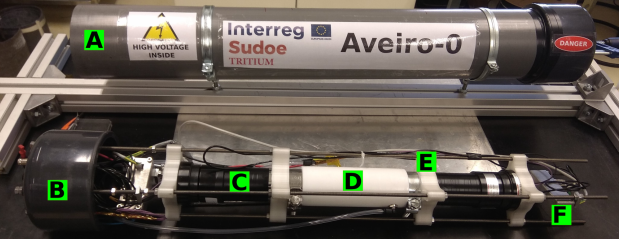
\includegraphics[scale=0.4]{5Prototypes/53FinalPrototypes/531TritiumAveiro/GeneralViewOfAveiroPrototype.png}
\caption{TRITIUM-Aveiro prototype.\label{fig:TritiumAveiro0}}
\end{figure}
 
\begin{figure}[h]
\centering
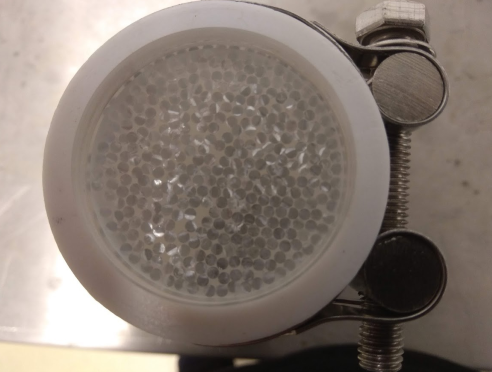
\includegraphics[scale=0.4]{5Prototypes/53FinalPrototypes/531TritiumAveiro/TeflonVessel_Fibers.png}
\caption{PTFE structure and fiber bundle used in TRITIUM-Aveiro prototype.\label{fig:TeflonStructureFibersTritiumAveiro0}}
\end{figure}
This vessel contains $360$ BCF-10 uncladded scintillating fibers of $180~\mm$ length from Saint-Gobain \cite{DataSheetBCF12Fiber}, which are similar to the BCF-12 fibers except the diameter, which is $2~\mm$. In order to quantify the importance of the fiber diameter, the measurements of this prototype are compared with similar measurements performed with the TRITIUM-IFIC-2 prototype. The scintillating fibers are stacked within the PTFE vessel in the maximum number that allows water to flow around them. These fibers were cleaved with the device described in section \ref{sec:CharacterizationScintillatingFibers}, but they were neither polished nor cleaned because the automatic polishing machine was not yet developed and it was not feasible to polish 360 fibers by hand. The PTFE vessel is totally closed and  a water inlet and outlet were installed to allow a constant water flux through it. Two PMMA $10~\mm$ thick windows, located at both ends of the fiber bundle, are used to read out the fibers. Two clamps are used to make a tight junction of the PTFE walls and the PMMA. PMMA was chosen for its optical properties, especially its transmission coefficient, which is larger than $95\%$ at the scintillating fiber wavelength. Two PMTs R2154-02 2" from Hamamatsu \cite{DataSheetPMTsAveiro}, shown in Figure \ref{fig:TritiumAveiro0}), are used to read out this prototype in coincidence. The HV was set at $-1500~\volt$ at which the quantum efficiency is $26\%$. These PMTs are attached to the vessel ends by two pieces, marked as E in Figure \ref{fig:TritiumAveiro0}, built with a 3D printer. They are optically coupled to the PMMA windows through optical grease \cite{OpticalGrease}. The Aveiro prototype and its electronics (marked as F in Figure \ref{fig:TritiumAveiro0}), were arranged in a structure composed of several clamps and four stainless-steel screws, locked to an external PVC structure, marked as A and B in Figure \ref{fig:TritiumAveiro0}, which protects the prototype from physical damage and provides a light-tight operation environment. This PVC structure is equiped with the necessary fed-through connectors. Only one prototype was built, which was designed to be installed in the Arrocampo dam. Two interfaces were developed to control the PMT power supply and the data adquisition. 

Measurements taken in the DRIM and LARUEX laboratories were used to characterize the detector. the prototype was in first place filled with pure water to measure the background and next with a radioactive liquid tritium solution of $30~\kilo\becquerel/\liter$ activity, which was used to measure the efficiency and the MDA of the prototype. The volume of pure water and tritium solution used in TRITIUM-Aveiro prototype was $58~\milli\liter$. 

%The energy distribution of single photons of the PMT dark current was measured. To avoid environmental light detection, the TRITIUM-Aveiro prototype was removed and the measurement was carried out only with the PMTs, the windows of which were covered with black caps. The output signal of the PMTs were digitalized, shaped and pulse-height measured by a CAEN V1724 digitalizer \cite{CAENV1724}. The single-photon energy distribution of both PMTs fitted to a Gaussian function, is shown in Figure \ref{fig:SinglePhotonEnergyDistribution}. Due to the electrical noise of the PMT, the low energy tail was extrapolated (dashed line).

%\begin{figure}[h]
%\centering
%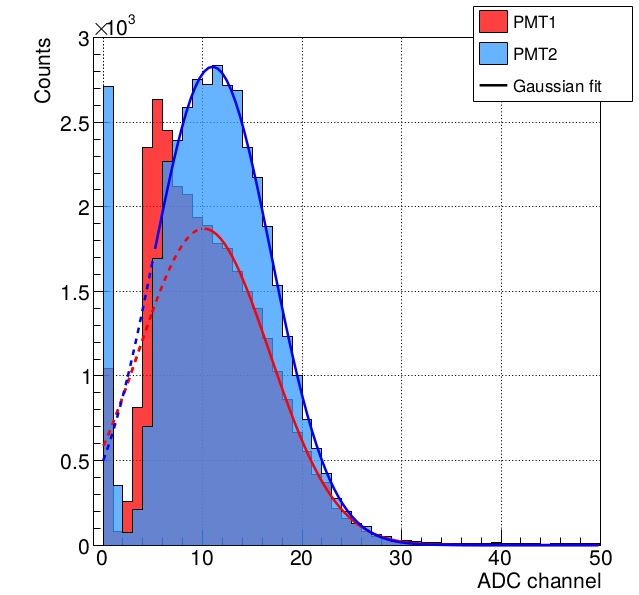
\includegraphics[scale=0.45]{5Prototypes/53FinalPrototypes/531TritiumAveiro/SinglePhotonEnergyDistribution.png}
%\caption{The single-photon energy distribution of both PMTs used in the TRITIUM-Aveiro prototype and their sum \cite{ExperimentalPaperCarlos}.\label{fig:SinglePhotonEnergyDistribution}}
%\end{figure}

%The distributions obtained deviates from Gaussian functions due to the noise in the low energy channels. As DRIM laboratory is not allowed to work with liquid radioactive source such as tritiated water, the first scintillating photons were produced by a $\ce{^{55}Fe}$ radioactive source since the energy of its $\gamma$ emission, $5.9~\keV$, is very close to the energy of tritium electrons. The TRITIUM-Aveiro prototype was coupled to both PMTs using optical grease and the radioactive source was placed inside the PTFE vessel. The prototype was not filled with water for this measurement. The spectra obtained are shown in Figure \ref{fig:55FeMeasurement}. A shift to higher energies is observed in the PMT2 data due to its higher gain and to the closer distance to the radioactive source.

%\begin{figure}[h]
%\centering
%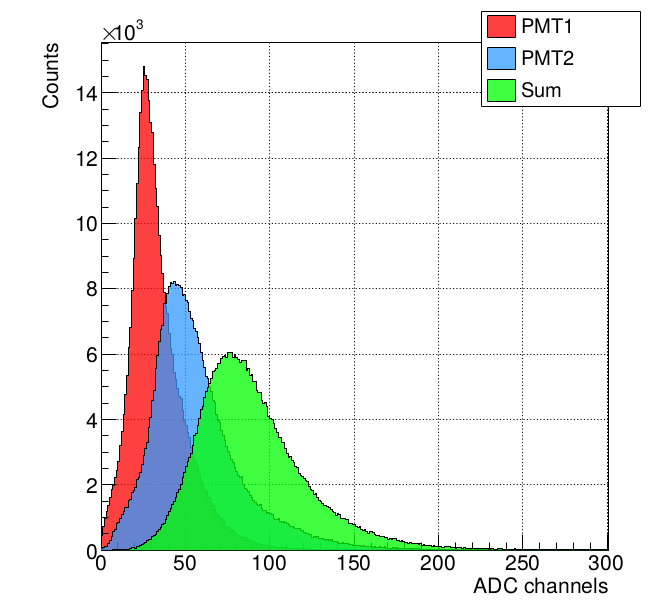
\includegraphics[scale=0.45]{5Prototypes/53FinalPrototypes/531TritiumAveiro/55FeMeasurement.png}
%\caption{Measurement of a $\ce{^{55}Fe}$ radioactive source with the TRITIUM-Aveiro prototype \cite{ExperimentalPaperCarlos}.\label{fig:55FeMeasurement}}
%\end{figure}


To quantify the background attenuation by a lead shield, measurements without shielding and with $2.5~\mm$ and $5~\mm$ lead shields were carried out. A background reduction by factors about 2 and 4 was obtained by the $2.5~\mm$ and $5~\mm$ lead shields, respectively, as shown in Figure \ref{fig:LeadShieldTest}.
\begin{figure}[h]
\centering
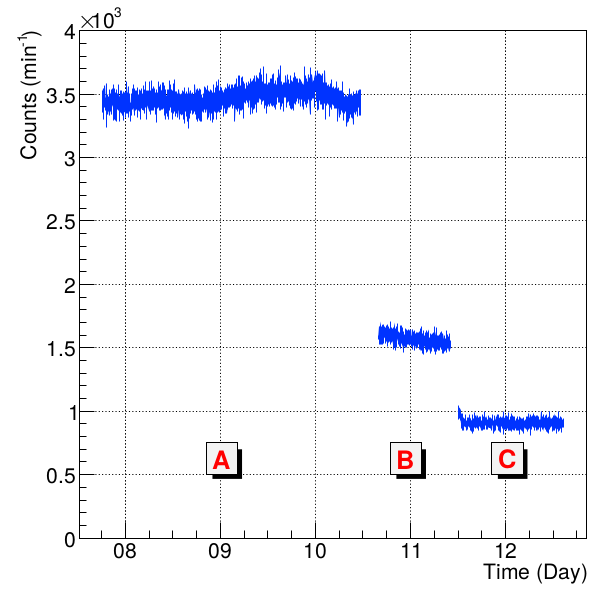
\includegraphics[scale=0.4]{5Prototypes/53FinalPrototypes/531TritiumAveiro/LeadShieldTest.png}
\caption{Background rate of the TRITIUM-Aveiro prototype. A) Without shielding. B) With a lead shield of $2.5~\mm$ thickness. C) With two lead shields of $2.5~\mm$ thickness each one \cite{ExperimentalPaperCarlos}.\label{fig:LeadShieldTest}}
\end{figure}
The prototype was installed in the LARUEX laboratory, at the University of Extremadura, in order to work with tritiated water. The background was measured during 4 days with the prototype filled with pure water and shielded by $5~\cm$ lead. The time adquisition of each measurement was $1$ minut. The data, fitted to a Gaussian function, are shown in Figure \ref{subfig:MeasurementInRealTime}. An average rate of $540$ counts/min with a standard deviation of $23$ counts/min was obtained. To calculate the Minimum Detectable Activity (MDA), the detection limit concepts developed by Lloyd A. Currie \cite{CurieLimit} were applied. The minimum number of net counts with a probability of a false-negative less than a $5\%$, is given by,
\begin{equation}
N_D = 4.65 \cdot{}\sigma_{Nb} + 2.71 = 108~\text{counts/min}
\label{eq:EquationNetCounts}
\end{equation}
which corresponds to a critical level of $Lc = 2.33\cdot{}\sigma_{Nb}=53 ~\text{counts/min}$. $L_C$ and $N_D$ refer to the net rate after background subtraction. Therefore, $L_C'$ and $N_D'$ referred to the detector signal before background subtraction are $593$ and $648$ counts/min respectively.
\begin{figure}
\centering
    \begin{subfigure}[b]{0.45\textwidth}
    \centering
    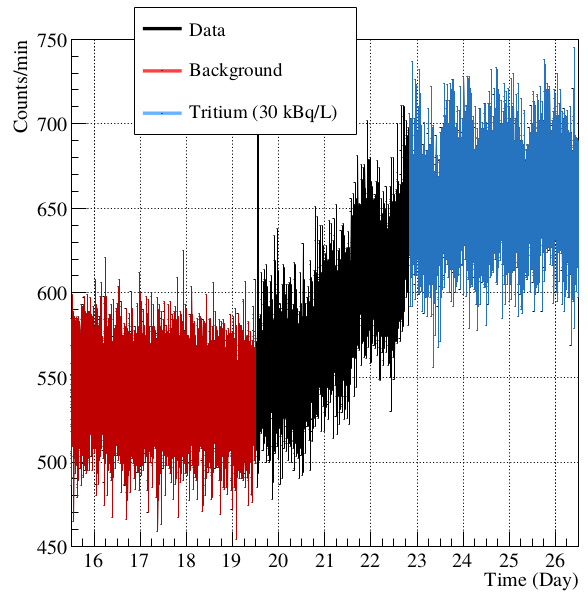
\includegraphics[width=\textwidth]{5Prototypes/53FinalPrototypes/531TritiumAveiro/Tritium_1min.png}  
    \caption{\label{subfig:MeasurementInRealTime}}
    \end{subfigure}
    \hfill
    \begin{subfigure}[b]{0.45\textwidth}
    \centering
    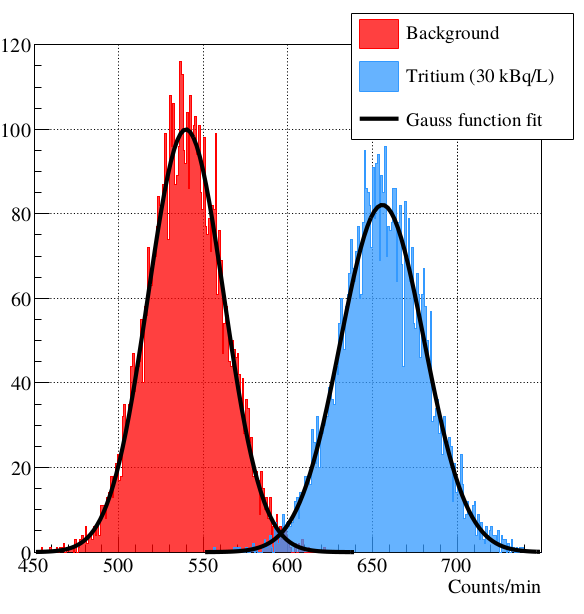
\includegraphics[width=\textwidth]{5Prototypes/53FinalPrototypes/531TritiumAveiro/Tritium_Gaus_1_min.png}  
    \caption{\label{subfig:DistributionofMeasurement}}
    \end{subfigure}
 \caption{Measurements of the background and tritium liquid source (with an activity of $29.8~\kilo\becquerel/\liter$) performed with the TRITIUM-Aveiro prototype and integred during a minute \cite{ExperimentalPaperCarlos}. a) Counts per minut measured as a function of time. b) Distribution of the acquired data.}
 \label{fig:BackgroundTritium1min}
\end{figure}
To find the MDA, tritiated water was slowly added  so that the tritium water activity increased continuously up to reach the $N_D'$ value. A rate of $656 \pm 26$ counts/min was obtained that corresponds to a MDA=$29.8~\kilo\becquerel/\liter$, measured with a Quantulus liquid scintillator system.

The tritium detection efficiency was calculated from the ratio of the net tritium rate measured, $1.9 \pm 0.6$ counts/sec, and the activity of the tritium source used, $29.8~\kilo\becquerel/\liter$. The efficiency obtained is $(6.5 \pm 1.9)\cdot{} 10^{-2}~\liter\:\kilo\becquerel^{-1}\second^{-1}$.  and the specific efficiency is
$$S=(1.6 \pm 0.5)\cdot{} 10^{-5}~\liter\:\kilo\becquerel^{-1}\second^{-1}\cm^{-2}$$ 
Comparing to the specific efficiency obtained with scintillating detectors (Table \ref{tab:PlasticScinTritium}) the specific efficiency of the TRITIUM-Aveiro prototype is close the largest value \cite{Hofstetter1, Hofstetter2} of $<2.22\liter\:\kilo\becquerel^{-1}/\second^{-1}\cm^{-2}$. The TRITIUM-Aveiro prototype has a lower specific efficiency than TRITIUM-IFIC-1, which could attribute to that the fibers in this prototype are neither polished nor cleaned. The efficiency uncertainty obtained for this prototype is larger than for first TRITIUM prototypes because the measurement time is shorter ($1$ minute) than the time used for the previous prototypes (several hours). Longer measurements are needed to quantify the reduction of the MDA of this prototype, which depends directly on the background uncertainty, equation \ref{eq:EquationNetCounts}. The data for an integrated time of $60$ minutes is shown in Figure \ref{fig:Tritium60min}. The mean and the uncertainty of the measured background data are $3.186 \cdot{} 10^{4}$ and $228$ counts per hour respectively. From the equation \ref{eq:EquationNetCounts}, values of $L_C=530$ and $N_D=1043$ counts per hour are obtained. Assuming linearity between the background and the tritiated water rates, $N_D'=3.872\cdot{}10^4$ counts per hour corresponds to a MDA of $4.53~\kilo\becquerel/\liter$. A daily oscillation is clearly observed in the Figure \ref{fig:Tritium60min}, indicating that the measurements are affected by external light. This oscillation begins on the $19^{th}$ day, when the water closed circuit pump was installed, so it is likely that the light tightness of the system was slightly.
\begin{figure}[h]
\centering
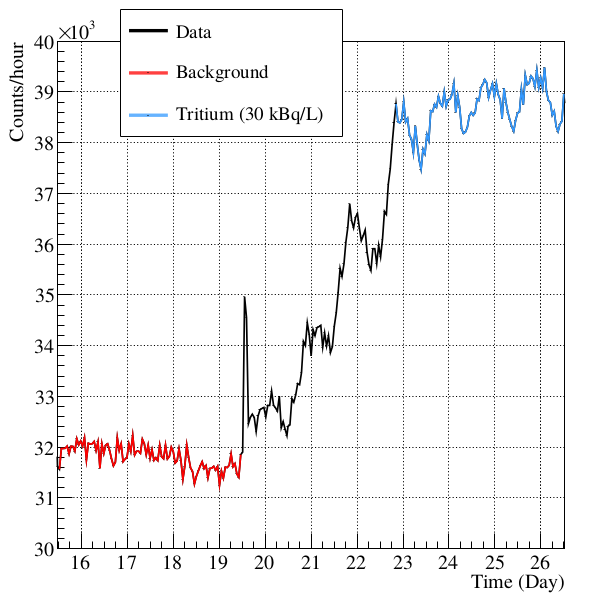
\includegraphics[scale=0.45]{5Prototypes/53FinalPrototypes/531TritiumAveiro/Tritium_60min.png}
\caption{Measurements of the background and tritium liquid source (with an activity of $29.8~\kilo\becquerel/\liter$) performed with the TRITIUM-Aveiro prototype and integrated during one hour \cite{ExperimentalPaperCarlos}.\label{fig:Tritium60min}}
\end{figure}
This prototype was finally installed in the Arrocampo dam to test its functionality and to begin with the tritium level monitoring reported in section \ref{sec:ResultsArrocampo}.